\documentclass[12pt,a4paper,article,english,firamath]{nsi}
\pagestyle{empty}
\begin{document}

\subsection*{Problem 1}

No hint.\\[4em]

\subsection*{Problem 2}

When a square's been removed, the number of remaining squares is odd.\\[4em]

\subsection*{Problem 3}

Start by covering the chessboard as simply as you can, then chose two adjacent squares to remove and see whaty you can do.\\[4em]

\subsection*{Problem 4}

Considere the chessboard as a closed path, following this figure :
\begin{center}
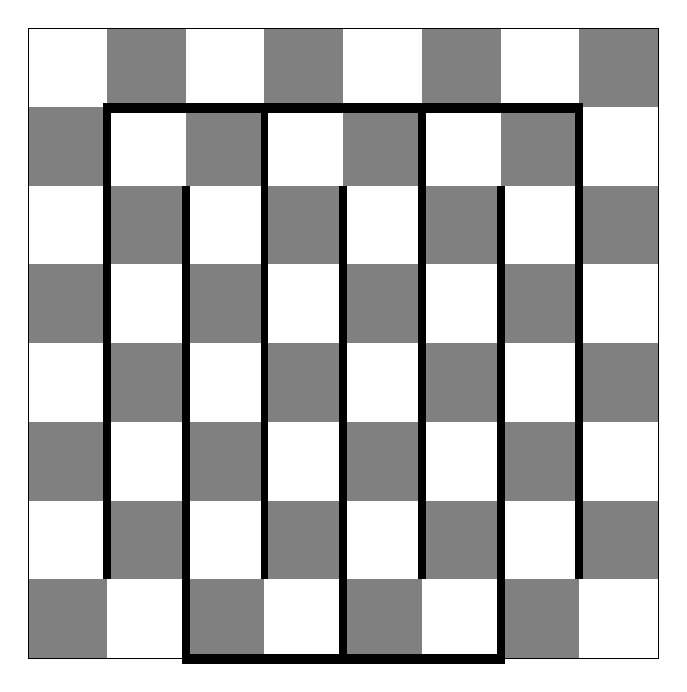
\begin{tikzpicture}
    \foreach \i in {0,1,...,7} {
      \foreach \j in {0,1,...,7} {
        \pgfmathtruncatemacro{\shade}{mod(\i+\j,2)}
        \ifnum\shade=0
          \fill[gray] (\i,\j) rectangle ++(1,1);
        \else
          \fill[white] (\i,\j) rectangle ++(1,1);
        \fi
      }
    }
    \draw (0,0) rectangle (8,8);
\foreach \i in {1,3,5,7} {
  \fill[black] (\i-.05,1) rectangle (\i+.05,7);
}
\foreach \i in {1,3,5}{\fill[black] (\i+1-.05,0) rectangle (\i+1.05,6);}
\fill[black] (1-.05,7-.075) rectangle (7.05,7.05);
\fill[black] (2-.05,-.075) rectangle (6.05,.05);
  \end{tikzpicture}\\[4em]
\end{center}

\subsection*{Problem 5}

Here, all you can do is find a counterexample.\\[4em]

\subsection*{Problem 6}

Have a look at this :
\begin{center}
  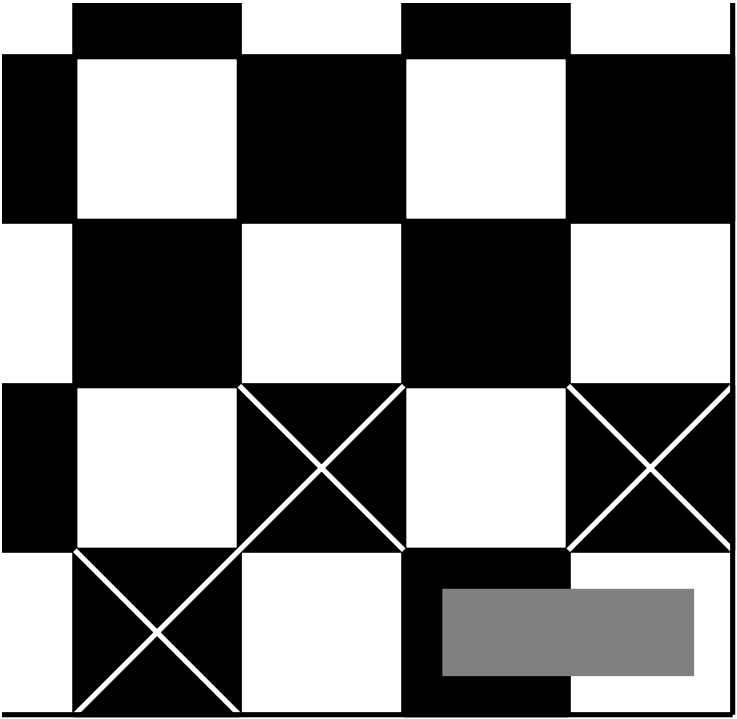
\includegraphics[width=7cm]{img/06}\\[4em]
\end{center}

\subsection*{Problem 7}

have a look at this :
\begin{center}
  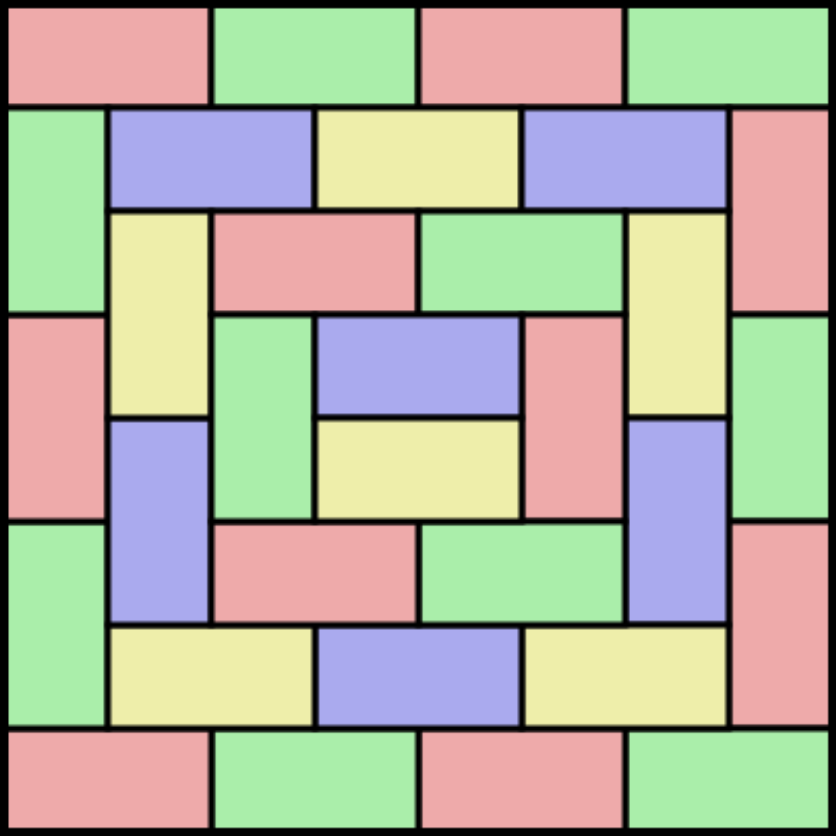
\includegraphics[width=7cm]{img/07}
\end{center}

\subsection*{Problem 8}

Consider one of the seven lines that separates two adjacent columns ; it divides the board into a left and a right part. We observe that 
\begin{enumerate}
  \item	because the column length is even, each column, and hence the left part, contains the same amount of black squares and white squares ;
  \item	because a domino consists of a blak and a white square, the dominoes entirely to
  the left of the line amount for an equal number of black and white squares.
\end{enumerate}

This should help.
% Combining the two observations, we conclude that, among the horizontal dominoes 
% crossed by the line, there are as many with a black left square as with a white one. Since each horizontal domino is crossed by exactly one of the seven lines, we conclude by summation that the number of horizontal dominoes with a black left square and the number of horizontal dominoes with a white left square are equal.
\end{document}